\chapter{ESTUDO DE CASO}

Este capítulo apresenta um estudo de caso com a avaliação do uso do \textit{Raspberry Pi} em um setor da Universidade Estadual do Norte Fluminense Darcy Ribeiro (UENF). Este estudo de caso foi idealizado para mensurar o quanto o equipamento apresentado pode ser útil para manipular o sistema informatizado do setor, avaliando assim o seu uso em ambientes de produção.

\section{Ambiente estudado}

O ambiente de produção escolhido para realizar a avaliação do Raspberry Pi foi a Assessoria de Suporte da UENF, setor responsável por atender as demandas da área de tecnologia da informação de toda a comunidade interna da universidade.

Durante a fase de criação deste estudo de caso o setor contava com cerca de 12 técnicos para atender às necessidades dos usuários, além do Sistema de Atendimento ao Usuários de TI, utilizado para gerenciar as solicitações de serviços por parte dos clientes. É um sistema dinâmico que permite ao solicitante a vantagem do acompanhamento do andamento da solicitação em tempo real, via email e \textit{online}.

Para acessar o sistema, cada técnico do setor possui disponível para si um pc desktop.

\section{Objetivo do estudo de caso}

O objetivo deste estudo de caso é realizar a avaliação do \textit{Raspberry Pi} como estação de trabalho utilizada pelos técnicos para acessar e manipular o sistema do setor. A opinião dos técnicos será recolhida por meio do preenchimento de um questionário, a fim de se mensurar o quanto o equipamento apresentado pode ser útil no ambiente de produção escolhido.

\section{Funções do sistema}

No segundo parágrafo serão descritos os passos que o usuário deve realizar para criar uma solicitação. Já no terceiro serão apresentadas as funções que o sistema deve fornecer ao técnico responsável por uma determinada solicitação. Vale lembrar que é sob a ótica do técnico de usar o sistema que o \textit{Raspberry Pi} será avaliado.

Ao detectar uma demanda em seu ambiente de trabalho que esteja relacionada à área de tecnologia da informação, o servidor da universidade deverá ser capaz de acessar o Sistema de Atendimento ao Usuários de TI e realizar uma solicitação ao setor de suporte.

Ao checar o recebimento de uma nova solicitação, o técnico deve poder interagir com ela, ou seja, ser capaz de inserir observações, alterar o status do andamento, cancelar, e etc, até chegar ao ponto de finalizá-la, momento que as demandas do usuário são totalmente atendidas.

\section{Uso do sistema através do \textit{Raspberry Pi}}

O teste do \textit{Raspberry Pi} será feito por 5 integrantes do setor. O tempo de uso de cada funcionário não será longo, pois o sistema utilizado por eles é relativamente pequeno, e oferece um número de funcionalidades que podem ser testadas no \textit{Raspberry Pi} em um curto período de tempo, a saber, cerca de 10 a 20 minutos.

O uso de \textit{Raspberry Pi} será realizado somente para executar as funcionalidades necessárias para o suprimento das demandas do setor, ou seja, para acessar o Sistema de Antendimento ao Usuário, e caso seja necessário, para acessar a caixa de emails.

\newpage

\section{Telas de exemplo do sistema}

\subsection{Tela 1 - Tela de \textit{login}}

\begin{figure}[ht]
    \centering
    \scalebox{0.6}{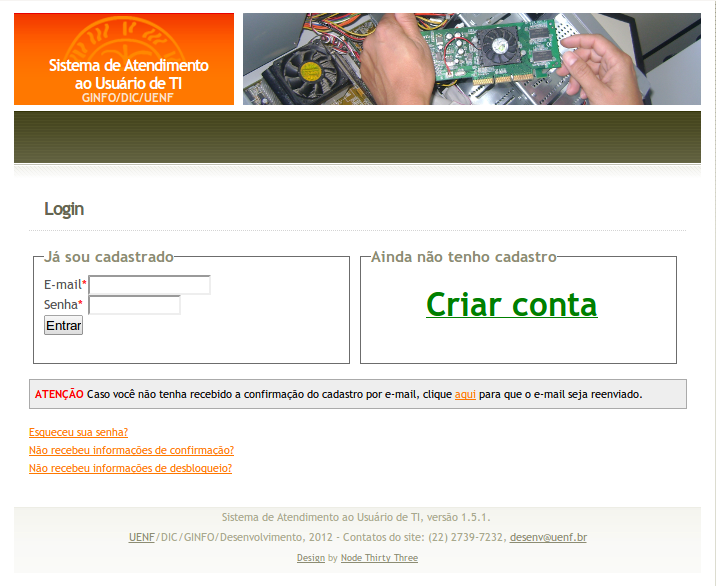
\includegraphics{figuras/login}}
    \caption{Tela de \textit{login} do sistema do setor}
\end{figure}

A Figura 6.1 apresenta a tela inicial do sistema. A tela deve ser carregada quando o endereço sistemas.uenf.br/suporte é acessado. Quanto o técnico inserir as informações de e-mail e senha, e clicar no botão ‘Entrar’, o sistema deverá carregar sua a página inicial, se o cadastro existir. Caso o técnico não tenha cadastro, o sistema deverá retornar uma mensagem avisando a não autenticação. Para ser criado um cadastro para um técnico é necessário comunicar com o responsável pelo desenvolvimento do sistema. Já para um solicitante, o cadastro é feito clicando no link ‘Criar conta’.

\newpage

\subsection{Tela 2 - Tela de dados pessoais}

\begin{figure}[ht]
    \centering
    \scalebox{0.6}{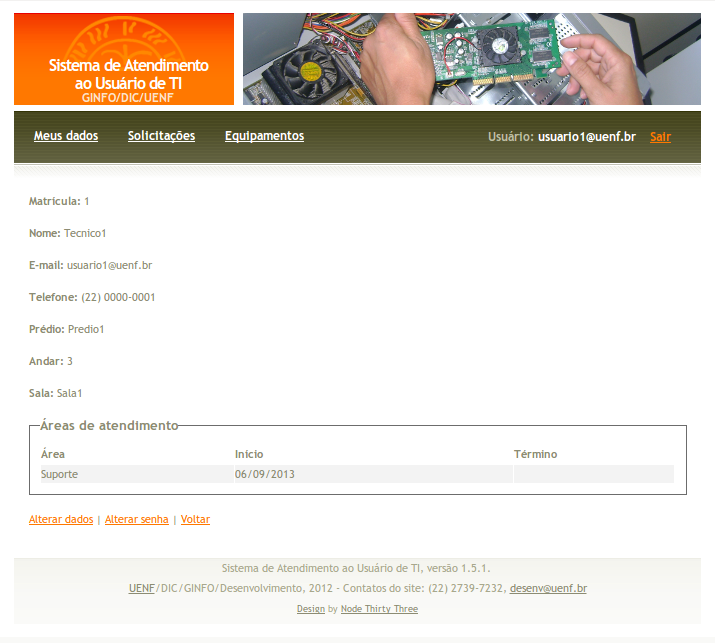
\includegraphics{figuras/home}}
    \caption{Tela inicial do técnico}
\end{figure}

A Figura 6.2 apresenta a tela inicial do técnico. Para carregá-la é preciso antes se autenticar no sistema através da tela representada na Figura 6.1. Nessa tela o técnico deverá poder visualizar e alterar seus dados pessoais bem como os referentes à sua área de atuação no setor. Quando alterada alguma informação e posteriormente enviadas para serem salvas, o sistema pode retornar erros de preenchimento segundo as críticas existentes, como por exemplo email inválido. 

\newpage

\subsection{Tela 3 - Tela das solicitações}

\begin{figure}[ht]
    \centering
    \scalebox{0.6}{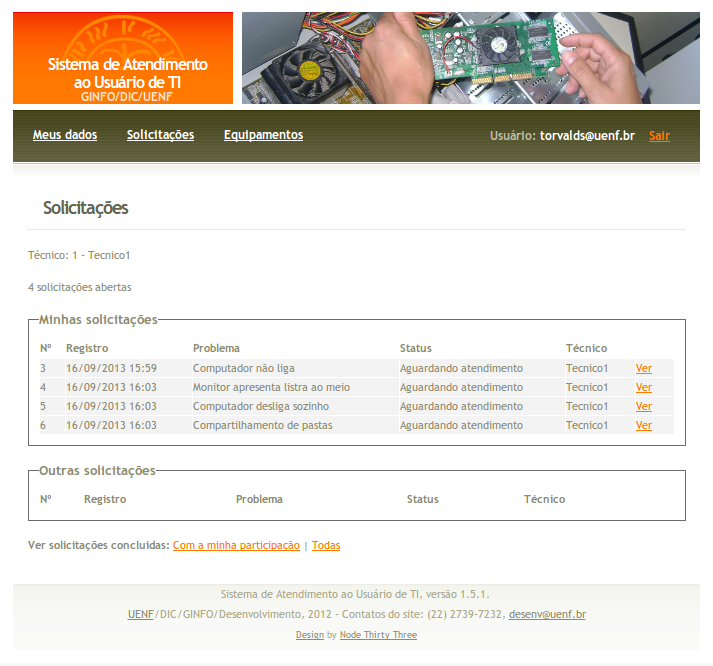
\includegraphics{figuras/solicitacoes}}
    \caption{Tela das solicitações}
\end{figure}

A Figura 6.3 representa a tela base das solicitações. Ela deverá ser carregada quando o técnico clicar no \textit{link} ‘Solicitações’ do menu de navegação, localizado na parte superior do sistema. A tela deverá apresentar, separadamente, todas as solicitações que estão sob a responsabilidade do técnico autenticado e as que estão sob a responsabilidade de outros técnicos. Ela também deverá permitir ao técnico visualizar as solicitações de forma específica. Ao clicar no \textit{link} ‘Ver’, presente na frente de cada solicitação, o sistema deverá carregar uma tela onde o técnico poderá checar todas as informações daquela solicitação. Nenhum erro pode ser gerado nessa tela.

\newpage

\subsection{Tela 4 - Tela de uma solicitação}

\begin{figure}[ht]
    \centering
    \scalebox{0.6}{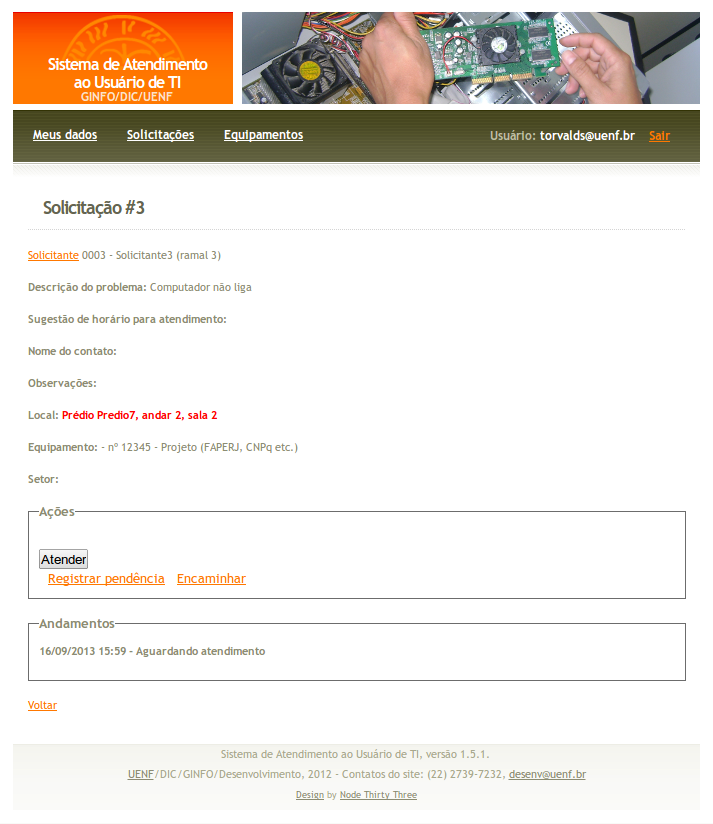
\includegraphics{figuras/solicitacao}}
    \caption{Tela de uma determinada solicitação}
\end{figure}

A Figura 6.4 apresenta a tela de uma determinada solicitação. Ela deverá ser carregada quando na tela representada pela Figura 6.3 o técnico clicar no \textit{link} ‘Ver’ presente na frente de cada solicitação. Esta tela deve fornecer ao técnico a possibilidade de execução de algumas ações em relação à solicitação, tais como ‘Atender’, ‘Registrar pendência’ ou ‘Encaminhar’. Ao clicar no \textit{link} ‘Atender’ deve surgir uma caixa de confirmação com a seguinte pergunta: ‘Esta solicitação entrará na fase de atendimento. Confirma?’; se o técnico clicar em ‘ok’, o sistema deverá carregar outras ações para a solicitação, como ‘Concluir’ e ‘Adicionar observação’.

\section{Execução do caso de uso}

O \textit{Raspberry Pi} foi utlizado segundo a tabela de dias e horários apresentada abaixo.

\begin{table}[!htpb]
 \centering
    \begin{tabular}{|p{2cm}|p{2cm}|p{2cm}|p{5cm}|p{2cm}|} 
    \hline
        \textbf{Dia} & \textbf{Usuário} & \textbf{Hora de início} & \textbf{Atividades realizadas} &  \textbf{Hora de término} \\
    \hline
         20/09/2013 & Técnico 1 & 15:33 & Técnico navegou pelas funcionalidades do sistema. & 15:45 \\
    \hline
        20/09/2013 & Técnico 2 & 15:57 & Além de navegar pelas funcionalidades do sistema, o técnico concluiu uma solicitação aberta. & 16:12 \\
    \hline
        20/09/2013 & Técnico 3 & 16:28 & Técnico navegou pelas funcionalidades do sistema. & 16:36 \\
    \hline
        20/09/2013 & Técnico 4 & 16:45 & Técnico navegou pelas funcionalidades do sistema e checou caixa de emails. & 17:03 \\
    \hline
        02/10/2013 & Técnico 5 & 12:33 & Técnico navegou pelas funcionalidades do sistema. & 12:46 \\
    \hline
    \end{tabular}
    \caption{Informações dos testes realizados pelos técnicos do setor}
    \label{t_fixa}
\end{table}

\section{Falhas durante a execução do caso de uso}

Durante a avaliação realizada pelos usuários não ocorreram falhas.

\section{Questionário}

O questionário tem como objetivo capturar o \textit{momento da verdade} de uso do dispositivo e apoiar a avaliação de sua adequação sob o ponto de vista dos usuários.

Abaixo de cada pergunta existiam cinco opções de resposta enumeradas de 1 a 5, e um texto de ajuda com a seguinte frase: “Assinale uma resposta entre 1 e 5, sendo 1 para a pior qualificação possível ou 5 para a melhor.”.
As perguntas foram apresentadas dessa forma:

\textbf{P1.} O hardware \textit{Raspberry Pi} é fácil de ser colocado em funcionamento?

\textbf{P2.} Você achou confortável o desempenho do equipamento ao executar o navegador (\textit{browser}) para acessar o site do sistema?

\textbf{P3.} Ao navegar pelo sistema e executar algumas de suas funcionalidades o desempenho do equipamento foi satisfatório?

\textbf{P4.} Como você avalia o equipamento com relação a travamentos quando executada alguma funcionalidade do sistema?

\textbf{P5.} Como você avalia o equipamento com relação a travamentos ocorridos em qualquer momento, seja utilizando as funcionalidades do sistema ou não?

\textbf{P6.} Levando em consideração somente a execução das funcionalidades pertinentes ao seu ambiente de produção, o quanto você acha viável a substituição de sua estação de trabalho por este equipamento avaliado?

\textbf{P7.} Dado que você precise de um computador para manipular um sistema semelhante ao do setor avaliado, o quanto você acha viável a utilização do equipamento apresentado?

\textbf{P8.} Levando em consideração a existência de um negócio seu que ainda não é informatizado, e sabendo que o preço de um \textit{Raspberry Pi} é  R\$ 176,02, o quanto o custo do equipamento apoia a ideia da criação de um sistema informatizado para gerenciar sua empresa?

\textbf{P9.} De um forma geral, você aprovou o equipamento avaliado?
